\section{Derivation of the Basic Model}
\label{section:derivation:basic_model}
\subsection{Predecessor: PCF Voltage Dynamics}
\begin{enumerate}
    \item Let $\tau_s$ be the synaptic time constant of each synapse in the network. Define dimensionless time as:
    \begin{equation*}
        \xi \overset{\Delta}{=} \frac{t}{\tau_s}.
    \end{equation*}\\
    We now assume our Linear Dynamical System is expressed in dimensionless time, i.e
    
    \begin{equation}
        \label{eq:lds_dimensionless}
        \frac{dx}{d\xi} = Ax(\xi) + B c(\xi).
    \end{equation}
    
    To describe the neuron dynamics in dimensionless time, let $o(\xi) \in \mathbf{R}^{N}$ be the spike trains of N neurons composing the network with components
    \begin{equation*}
        o_j(\xi) = \sum_{k=1}^{\text{$n_j$ spikes}} \delta(\xi - \xi_{j}^{k}),
    \end{equation*}
    where $\xi_j^k$ is the time at which neuron $j$ makes its $k^{th}$ spike. 
    Define the network's estimate of the state variable as
    \begin{equation}
        \label{eq:xhat}
        \hat{x}(\xi)
        \overset{\Delta}{=} D r(\xi), 
    \end{equation}
    where $D \in \mathbf{R}^{d \times N}$ and 
    \begin{equation}
    \label{eq:rdot}
        \frac{dr}{d \xi} = -r + o(\xi).
    \end{equation}\\
    When the probability of synaptic transmission is $1$, component $r_j$ is the total received post-synaptic current (PSC) from neuron $j$ by the network estimator. 
    Define the network error as
    \begin{equation}
    \label{eq:error_def}
        e(\xi) \overset{\Delta}{=} x(\xi) - \hat{x}(\xi).
    \end{equation}
    
    \item From equations (\ref{eq:rdot}) and (\ref{eq:xhat}), we have
    
    \begin{align*}
        D \dot{r} + D r &= Do \\
        \\
        \implies \dot{\hat{x}} + \hat{x} &= Do,
    \end{align*}
    where the dot denotes derivative w.r.t dimensionless time $\xi$.

    Subtract $\dot{\hat{x}}$ from $\dot{x}$ to get $\dot{e}$:
	\begin{align*}
        \dot{e} &= \dot{x}-\dot{\hat{x}} \\
        &= \left( Ax + Bc \right) - \left( Do - \hat{x} \right) \\
        &= A\left(  e + \hat{x} \right) + Bc - Do + \hat{x} \\
        &= A e + (A + I)\hat{x} + Bc - Do \\
        &=  A e + (A + I) \left(Dr\right) + Bc - Do  \\
        \implies D^T \dot{e} &= D^T A e + D^T (A + I) \left(Dr\right) + D^T Bc - D^T Do. 
	\end{align*} 
	
The quantity $D^T e$ defines the membrane voltage of the predictive coding framework (PCF), a precursor to this model:
$$
	v_{pcf} \overset{\Delta}{=}  D^T e.
$$
Note that the definition implies $e = D^{T \dagger} v_{pcf}$. 
The voltage dynamics are thus

\begin{align}
\label{eq:derivation_init}
\dot{v}_{pcf} 
= 
D^T A D^{T \dagger} v_{pcf} + D^T (A + I) \left(Dr\right) + D^T Bc - D^T Do,
\end{align}

where $D^{T \dagger}$ is the left pseudo-inverse of $D^T \in \mathbf{R}^{N \times d}$. The PCF thus defines a mapping between two vector spaces: the d-dimensional state space of the target system, and the N-dimensional voltage space of the spiking neural network. This mapping is visualized in figure (\ref{fig:derivation:basic_model:pcf_e_v_map}). 
\begin{figure}
    \centering
    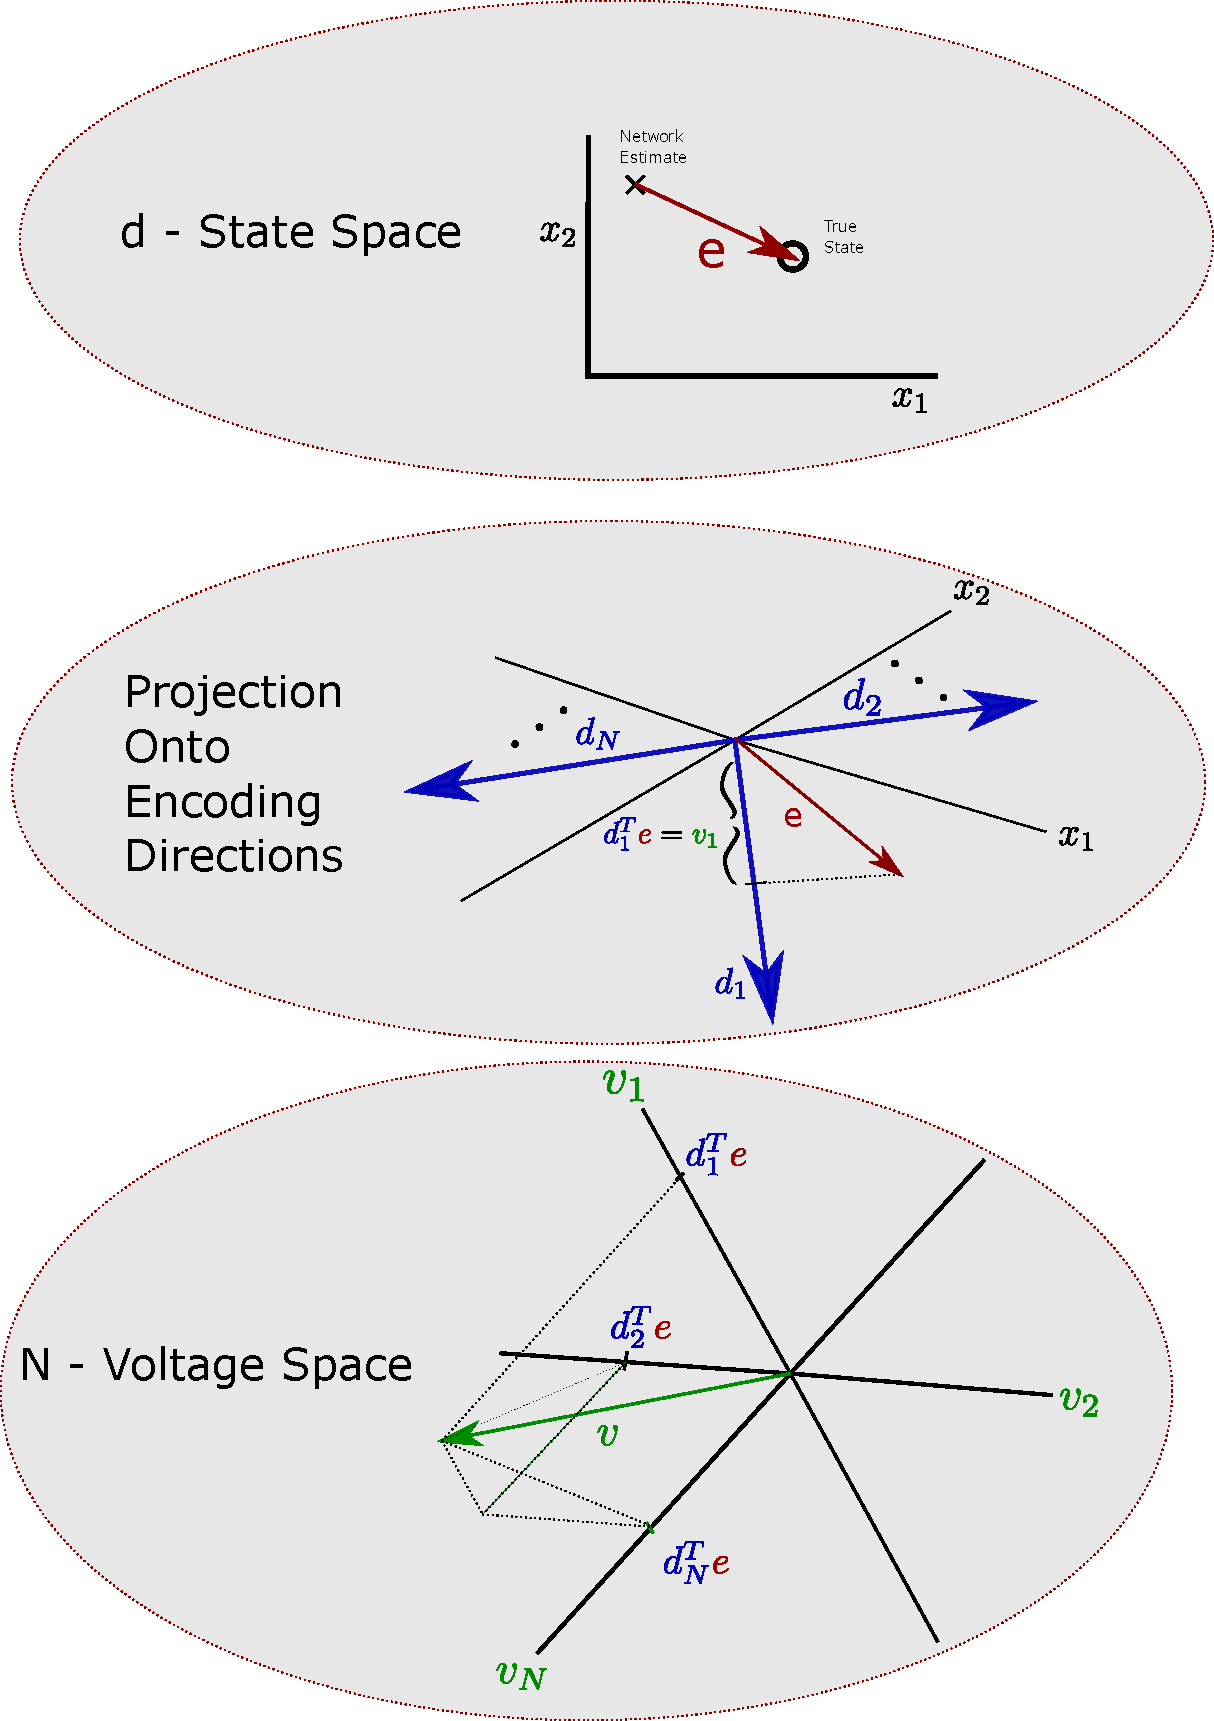
\includegraphics[scale=.703]{figures/pcf_e_v_graphic.pdf}
    \caption{Mapping Between State and Voltage Spaces: \textbf{\textit{Top:}} The estimation error $e$ is computed by comparing the decoded network estimate to the true state of the target dynamical system.  \textbf{\textit{Middle:}} The $e$ is projected onto the encoding directions of the neurons composing the network. The projection of error onto encoding direction $j$ gives the membrane voltage of neuron $j$, $v_j = d_j^T e$. \textbf{\textit{Bottom:}} The voltages form a N-dimensional vector contained in voltage space.}
    \label{fig:derivation:basic_model:pcf_e_v_map}
\end{figure}

\end{enumerate}

\clearpage

\subsection{The Self-Coupled Model is PCF in an Orthonormal Basis}
\begin{enumerate}
\item The self-coupled network is derived from the PCF via a change of bases. Assuming both $D$ and $A$ are full rank, diagonalize each to a common left basis:
\begin{align*}
    A &= \mathcal{U} \Lambda \mathcal{U}^T = \sum_{j=1}^d \Lambda_j \mathcal{U}_j \mathcal{U}_j^T,\\
    \\
    D &= \mathcal{U} \left[S \hspace{2mm} 0 \right]  V^T = \sum_{j=1}^d S_j \mathcal{U}_j  V_j^T,\\
    \\
    D^T &= V \begin{bmatrix} S \\ 0\end{bmatrix} \mathcal{U}^T = \sum_{j=1}^d S_j V_j  \mathcal{U}_j^T, \\
    \\
    D^T D  &= V \begin{bmatrix} S \\ 0\end{bmatrix} \begin{bmatrix} S & 0\end{bmatrix} V^T
     = \sum_{j=1}^d S_j^2 V_j V_j^T , 
\end{align*}
with $\mathcal{U} \in \mathbf{R}^{d \times d}$ and $V \in \mathbf{R}^{N \times N}$, and $S \in \mathbf{R}^{d \times d }$. \\
\\

In the original basis, the state is $x$. In the rotated basis we denote this quantity as $y$. It is the projection of $x$ onto the d-dimensional $\mathcal{U}$ basis:

\begin{align}
\label{eq:definition_rotated_state_space}
y &\overset{\Delta}{=} \mathcal{U}^T x 
%\hat{y} &\overset{\Delta}{=} \mathcal{U}^T \hat{x}.
\end{align}

The rotated target dynamics are thus

\begin{align}
\label{eq:rotated_targed_dynamical_system}
\dot{y} &= \mathcal{U}^T \dot{x} \notag
\\ \notag
\\ \notag
&= 
\Lambda y (\xi)
+
\mathcal{U}^T B c(\xi)
\\ \notag
\\ \notag
&= 
\Lambda y (\xi)
+
\mathcal{U}^T B \mathcal{U} \mathcal{U}^T c(\xi) \notag
\\ \notag
\\ 
&=
\Lambda y (\xi)
+
\beta \tilde{c}(\xi)
\end{align}
where  
$$
\beta \overset{\Delta}{=} \mathcal{U}^T B \mathcal{U},  
$$
and
$$
\tilde{c} \overset{\Delta}{=} \mathcal{U}^T c,
$$
give the projections of $B$ and $c$ respectively.
The network estimate in the rotated basis is 
$$
\hat{y} \overset{\Delta}{=} \mathcal{U}^T \hat{x}.
$$

From equation (\ref{eq:xhat}),
\begin{align*}
\hat{y} &= \mathcal{U}^T \hat{x}
\\ 
\\ 
&=
\mathcal{U}^T D r
\\ 
\\ 
&= 
\begin{bmatrix}
S & 0
\end{bmatrix}
V^T
r
\\
\\
&=
\begin{bmatrix}
S & 0
\end{bmatrix}
\rho
\\
\\
\implies
\dot{\hat{y}}
&= 
\begin{bmatrix}
S & 0
\end{bmatrix}
V^T
\dot{r}
\\
\\
&= 
\begin{bmatrix}
S & 0
\end{bmatrix}
\left( 
-V^T r + V^T o
\right).
\end{align*}

Note that $V^T r$ and $V^T o $ are projections of the N-neuron network's post-synaptic current and spike train respectively onto the rotated basis, denoted by 

\begin{align}
\rho \overset{\Delta}{=} V^T r, 
\label{eq:def_rho}
\\ \notag
\\
\tilde{o} \overset{\Delta}{=} V^T o
\label{eq:def_o_tilde}.
\end{align}

The preceding equality also gives $\hat{y}$ in terms of $\rho$:

\begin{align}
\label{eq:basic:def:y_hat}
\hat{y} = 
\begin{bmatrix}
S & 0
\end{bmatrix}
\rho.
\end{align}

With these definitions, the last equality above also implies

\begin{align}
\label{eq:rho_dot}
\dot{\rho} = -\rho + \tilde{o}.
\end{align}

To finish describing the basic network quantities in terms of the rotated basis, let $\epsilon$ be the error in the rotated basis:
\begin{align}
\label{eq:rotated_error_def}
\epsilon \overset{\Delta}{=} y - \hat{y} \\= \mathcal{U}^T e. \notag
\end{align}

\item Repeat the derivation of equation (\ref{eq:derivation_init}) but with $y$, $\hat{y},$ and $\epsilon$:

\begin{align*}
\dot{\epsilon}
&=
\dot{y} - \dot{\hat{y}}
\\
\\
&= 
\Lambda y + \beta c - 
\begin{bmatrix}
S & 0
\end{bmatrix}
\left(
-\rho + \tilde{o}
\right)
\\
\\
&= 
\Lambda \left(
\epsilon + 
\begin{bmatrix}
S & 0
\end{bmatrix}
\rho
\right)
+ 
\beta tilde{c}
-
\begin{bmatrix}
S & 0
\end{bmatrix}
\left(
-\rho + \tilde{o}
\right)
\\
\\
&= 
\Lambda \epsilon
+
\left( 
\Lambda + I
\right)
\begin{bmatrix}
S & 0
\end{bmatrix}
\rho
+ 
\beta \tilde{c}
-
\begin{bmatrix}
S & 0
\end{bmatrix}
\tilde{o}
\\
\\
\implies
\begin{bmatrix}
S \\ 0
\end{bmatrix}
\dot{\epsilon}
&= 
\begin{bmatrix}
S \\ 0
\end{bmatrix}
\Lambda \epsilon
+
\begin{bmatrix}
S \\ 0
\end{bmatrix}
\left( 
\Lambda + I
\right)
\begin{bmatrix}
S & 0
\end{bmatrix}
\rho
+
\begin{bmatrix}
S \\ 0
\end{bmatrix}
\beta
\tilde{c}
-
\begin{bmatrix}
S \\ 0
\end{bmatrix}
\begin{bmatrix}
S & 0
\end{bmatrix}
\tilde{o}.
\end{align*}

The last equality gives a system of $N$ equations of which only $d$ are nontrivial. A comparison with equation (\ref{eq:derivation_init}) suggests the N-dimensional rotated membrane potential $v$ is best defined as:

\begin{align}
\label{eq:rotated_voltage_def}
v \overset{\Delta}{=} \begin{bmatrix}
S \\ 0
\end{bmatrix} \epsilon \in \mathbf{R}^N.
\end{align}
\\
This mapping is invertible from $v$ to $\epsilon$ if we write  
$$
\epsilon = \begin{bmatrix} S^{-1} & 0 \end{bmatrix}.
$$
This gives a well-defined $d-$vector. whose first $d$ elements are well defined, and the remaining components of $v$ are assumed to be zero. Using a similar abuse for the $\rho$ and $\tilde{o}$ terms, we arrive at the system of $N$ equations describing the network voltage dynamics:
\begin{align}
\label{eq:rotated_voltage_dynamics}
\dot{v}
&= 
\begin{bmatrix}
\Lambda & 0
\\
0 & 0
\end{bmatrix}
v +
\begin{bmatrix}
S \left(\Lambda + I_d \right) S & 0
\\
0 & 0
\end{bmatrix}
  \rho 
  +
\begin{bmatrix}
S \\ 0
\end{bmatrix}  
\beta \tilde{c}
  - 
 \begin{bmatrix}
S^2 & 0
\\
0 & 0
\end{bmatrix}
    \tilde{o}.
\end{align}

To summarize conceptually, there are 4 vector spaces in total: the error space which tracks the dynamical system and the network estimate, the voltage space which tracks the membrane potentials, and the transformed counterparts of each in the $\mathcal{U}-V$ bases. Figure (\ref{fig:four_subspace_relation}) shows the relationships derived between these subspaces.

\begin{figure}[h]
\centering
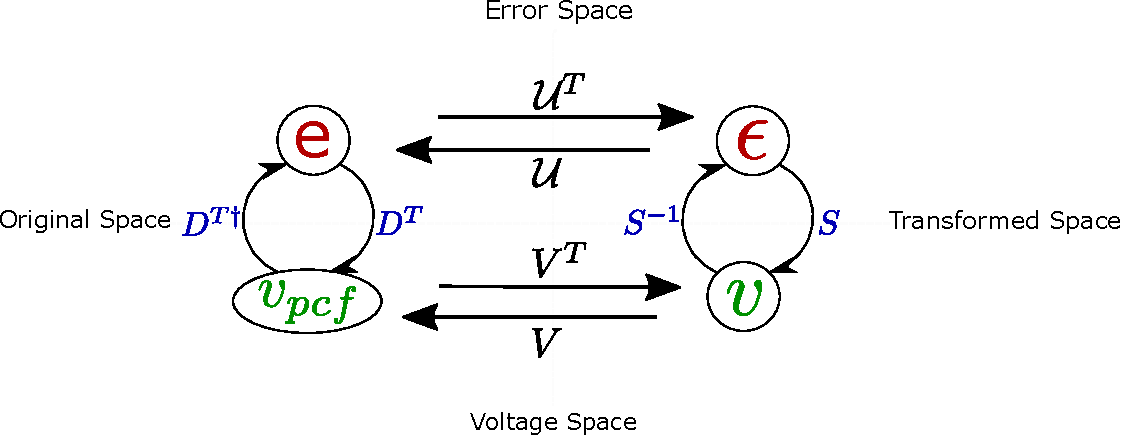
\includegraphics[width=\linewidth]{figures/ev_rotated_classic_graph}
\caption{Depiction of the relationship between original and transformed spaces and their respective error and voltage spaces. An arrow represents left multiplication by the given matrix. The zeros in the full $N \times N$ matrices mapping between $v$ and $\epsilon$ are omitted for clarity.}
\label{fig:four_subspace_relation}
\end{figure}
\end{enumerate}   
\clearpage
   
\subsection{Optimizing Spike-Timing: From PCF to Self-Coupled} 

\begin{enumerate}
\item In PCF, the spike trains $o$ are chosen minimize the network estimation error
\begin{align}
    \mathcal{L}(\xi) =  || x(\xi + d\xi) - \hat{x}(\xi + d\xi) ||^2. 
\end{align}
The network greedily minimizes $\mathcal{L}(\xi)$ an instant $d\xi$ ahead in time. If no spike occurs at time $\xi$, then the objective is given above. If neuron $j$ spikes, the estimate $\hat{x} \leftarrow \hat{x} + d_j$, where $d_j$ is column $j$ of $D$. The objective is now

\begin{align*}
\mathcal{L}_{sp}(\xi) &= ||x - (\hat{x} + d_j)||^2
\\
\\
&= x^T x - 2 \, x^T \hat{x} - 2 x^T d_j + \hat{x}^T \hat{x} + 2 \hat{x}^T d_j + d_j^T d_j
\\
\\
&= x^T x - 2 x^T \hat{x} + \hat{x}^T \hat{x} - 2 d_j^T(x - \hat{x}) + d_j^T d_j
\\
\\
&= ||x - \hat{x}||^2 - 2 d_j^T(x - \hat{x}) + d_j^T d_j
\\
\\
&= 
\mathcal{L}_{ns}(\xi) - 2 d_j^T(x - \hat{x}) + d_j^T d_j,
\end{align*}
where $\mathcal{L}_{ns}(\xi)$ is the objective if no spike occurs. Spiking occurs when the objective decreases or
\begin{align*}
\mathcal{L}_{sp} &< \mathcal{L}_{ns}
\\
\\
\implies
- 2 d_j^T(x - \hat{x}) &+ d_j^T d_j < 0
\\
\\
\implies
d_j^T(x - \hat{x}) >& \frac{||d_j||^2}{2}.
\end{align*}
Since $d_j^T(x-\hat{x}) = d_j^Te$ is already defined as membrane voltage, the right hand side gives neuron $j's$ spike threshold voltage $v_th$,

$$
v_{th}^{pcf} = \frac{1}{2}
\begin{bmatrix}
d_1^T d_1
\\
\vdots
\\
d_N^T d_N
\end{bmatrix}.
$$

\item For the rotated network, note $\mathcal{U}^T$ is an orthonormal matrix by definition. Thus it is norm-preserving:

\begin{align*}
\mathcal{L}_{sp}(\xi) &= ||x - \hat{x}||^2
\\
\\
&= 
||\mathcal{U}^T(x - \hat{x})||^2
\\
\\
&= 
||y - \hat{y}||^2.
\end{align*}

If we define the rotated network objective as 
$$
\tilde{L}(\xi) \overset{\Delta}{=} || y(\xi + d\xi) - \hat{y}(\xi + d\xi)||^2,
$$
it is equal to the original network objective when no spike occurs. However, a spike alters the readout by $\hat{y} \leftarrow \hat{y} + S_l$, where $S_l$ is the $l^{th}$ column of $\begin{bmatrix}
S & 0
\end{bmatrix}$. With the same approach as above, the objective when neuron $l$ spikes is

\begin{align*}
\tilde{L}_{sp} &= \tilde{L}_{ns} + 2 S_l^T\epsilon  + S_l^TS_l
\\
\\
\implies
v_l &> \frac{||S_l||^2}{2}.
\end{align*}

This leads to voltage thresholds

$$
v_{th} = \frac{1}{2}
\begin{bmatrix}
S_1^TS_1
\\
\vdots
\\
S_d^T S_d
\\
0
\\
\vdots
\\
0
\end{bmatrix}. 
$$

\end{enumerate}

\subsection{Consequences of Positive Unit-Area Spikes}
\begin{enumerate}
\item The voltage thresholds are nonnegative, such that neuron $j$ will only spike if 

$$
v_l = S_l^T \epsilon > v_{th} > 0.
$$

The spike form neuron $l$ corrects the network error $\epsilon$ by adding $S_l$ to the estimate $\hat{y}$. The nonnegative voltage implies it is impossible for neuron $l$ to correct antiparallel errors ($-S_l$), since
$$
S_l^T(\epsilon) = S_l^T(-S_l) = - ||S_l||^2 < 0 < v_{th}.
$$

To illustrate consider the space of errors $\epsilon \in \mathbf{R}^d$ which satisfy the voltage threshold of neuron $l$, i.e
$$ 
\epsilon_{sp} = \left\{ \epsilon \in \mathbf{R}^d \, | \, S_l^T \epsilon > v_{th}  \right\}. 
$$

In $\mathbf{R}^2$, $\epsilon_{sp}$ is the half-plane formed by the line normal to $S_l$ shifted $v_{th}$ from the origin along $S_l$ as in figure (\ref{fig:relu_encoding_demo}). This excludes $-S_l$. The optimization thus tells us that neuron $l$ spikes when the projection $S_l^T\epsilon$ exceeds $v_{th}$. 


\begin{figure}
\centering
\includegraphics[scale=.5]{figures/half_plane_relu_demo}
\caption{Sketch of the Encoding space $\epsilon_{sp}$ of neuron $l$ with direction $S_l \in \mathbf{R}^2.$ The radius of the circle is $v_{th}=\frac{||S_l||^2}{2}$. (Vector $S_l$ not drawn to scale).}
\label{fig:relu_encoding_demo}
\end{figure} 

\clearpage


\item Equations (\ref{eq:rotated_voltage_dynamics}) and (\ref{eq:rho_dot}) describe how we implement a network with d neurons that produces an estimate $\hat{y}$ of the given target system. As written, the network can only encode vectors $y$ with strictly nonnegative elements. To see why we return to the optimization procedure performed by the network. 

The network optimizes the objective 

$$
\mathcal{L} = || y - \hat{y}||,
$$

by choosing spike times $\tilde{o}$. The spikes are integrated into a post-synaptic feedback $\rho$. This feedback vector is scaled by $S$ to generate the estimate $\hat{y}$ that minimizes the objective at time $\xi$.  In other words, the network performs the optimization

$$
\underset{\rho \in \mathbf{R}^{d+}}{min} ||y - S \rho ||^2,
$$

where $\mathbf{R}^{d+}$ denotes the real $d-$vectors with nonnegative components. The components must be nonnegative because the spikes $\tilde{o}$ have nonnegative area when integrated, and their dynamics will not decay below zero otherwise. In using a greedy approach with only one spike at a given time step, the network more specifically performs 
$$
\underset{x \in \mathbf{Z}^{d+} \, : \, \sum_j Z_j = 1}{min} ||y - S \left( \rho + x\right) ||^2.
$$

I.e, it must choose one neuron to spike with unit area 1, which adds precisely one column of $S$ to the estimate $\hat{y}$. 

It is easier to analyze the former optimization of $\rho \in \mathbf{R}^{d+}$, and we do so here. Because $ \left\{x \in \mathbf{Z}^{d+} \, : \, \sum_j Z_j = 1 \right\} \subset \mathbf{R}^{d+},$ it is always the case that 
$$
\underset{\rho \in \mathbf{R}^{d+}}{min} ||y - S \rho ||^2
\leq \underset{x \in \mathbf{Z}^{d+} \, : \, \sum_j Z_j = 1}{min} ||y - S \left( \rho + x\right) ||^2,
$$

i.e optimizing over arbitrary $ \rho \in \mathbf{R}^{d+}$ will always give just as low or lower objectives than under the single-greedy spike optimization.

We're interested in the range of vectors representable by the network.  That is the set

$$
X^* = \left\{x \in  \mathbf{R}^{d+} \, \ : \, Sx = y \right\}.
$$


Over this set, the objective function is 0, i.e. 
$$
X^* = \left\{x \in  \mathbf{R}^{d+} \, \ : \, \mathcal{L}=||y-Sx||^2 = 0 \right\}. 
$$

Let $x \in X^*$, and consider its negative $-x$. It follows that 

\begin{align*}
x &= S\rho
\\
\\
\implies -x &= -S \rho
\\
\\
&= S \left(-\rho\right). 
\end{align*}

However if $\rho \in \mathbf{R}^{d+}$, then it is impossible for $-\rho \in \mathbf{R}^{d+}$ to also be true. Thus $-\rho \not\in X^*$ so that $\mathcal{L} > 0$. We conclude that for any vector $\hat{y}$, the network can represent with $\mathcal{L}=0$, there exists a negative vector that the network cannot represent with $\mathcal{L}=0$. This is undesirable as it restricts the set of vectors the network can reconstruct within a given error tolerance. In $\mathbf{R}^2$ for example, network representation where $\mathcal{L} = 0$ is restricted to the first quadrant. This restriction applies equally to the greedy single-spike optimization. 

This issue is unique to the self-coupled network and does not occur in the original PCF network even through its spikes must also have positive unit area. The difference arises when we take the SVD of the decoder matrix.
$$
D = \mathcal{U} \begin{bmatrix} S & 0 \end{bmatrix} V^T.
$$ 

The SVD decomposes $D$ into orthonormal bases $\mathcal{U}$ and $V$ which are mapped to one another by singular values $S$, as in figure (\ref{fig:linear_maps_between_subspaces_D_real}). By rotating into the $\mathcal{U}-V$ bases, we preemptively perform the first and last mappings, leaving only multiplication by a diagonal matrix. This eliminates linearly dependent encoding vectors, keeping only the orthonormal. For example, suppose $x = Dy = \mathcal{U} \begin{bmatrix} S & 0 \end{bmatrix} V^T y$. For an orthonormal basis, $-x$ is obtainable by $\mathcal{U} \begin{bmatrix} S & 0 \end{bmatrix} V^T (-y)$. However the constraint that spikes have positive unit area prevents a vector $\rho=-y$ from being reachable by the network as written. We consider two options to address this below.  




\begin{figure}
\centering
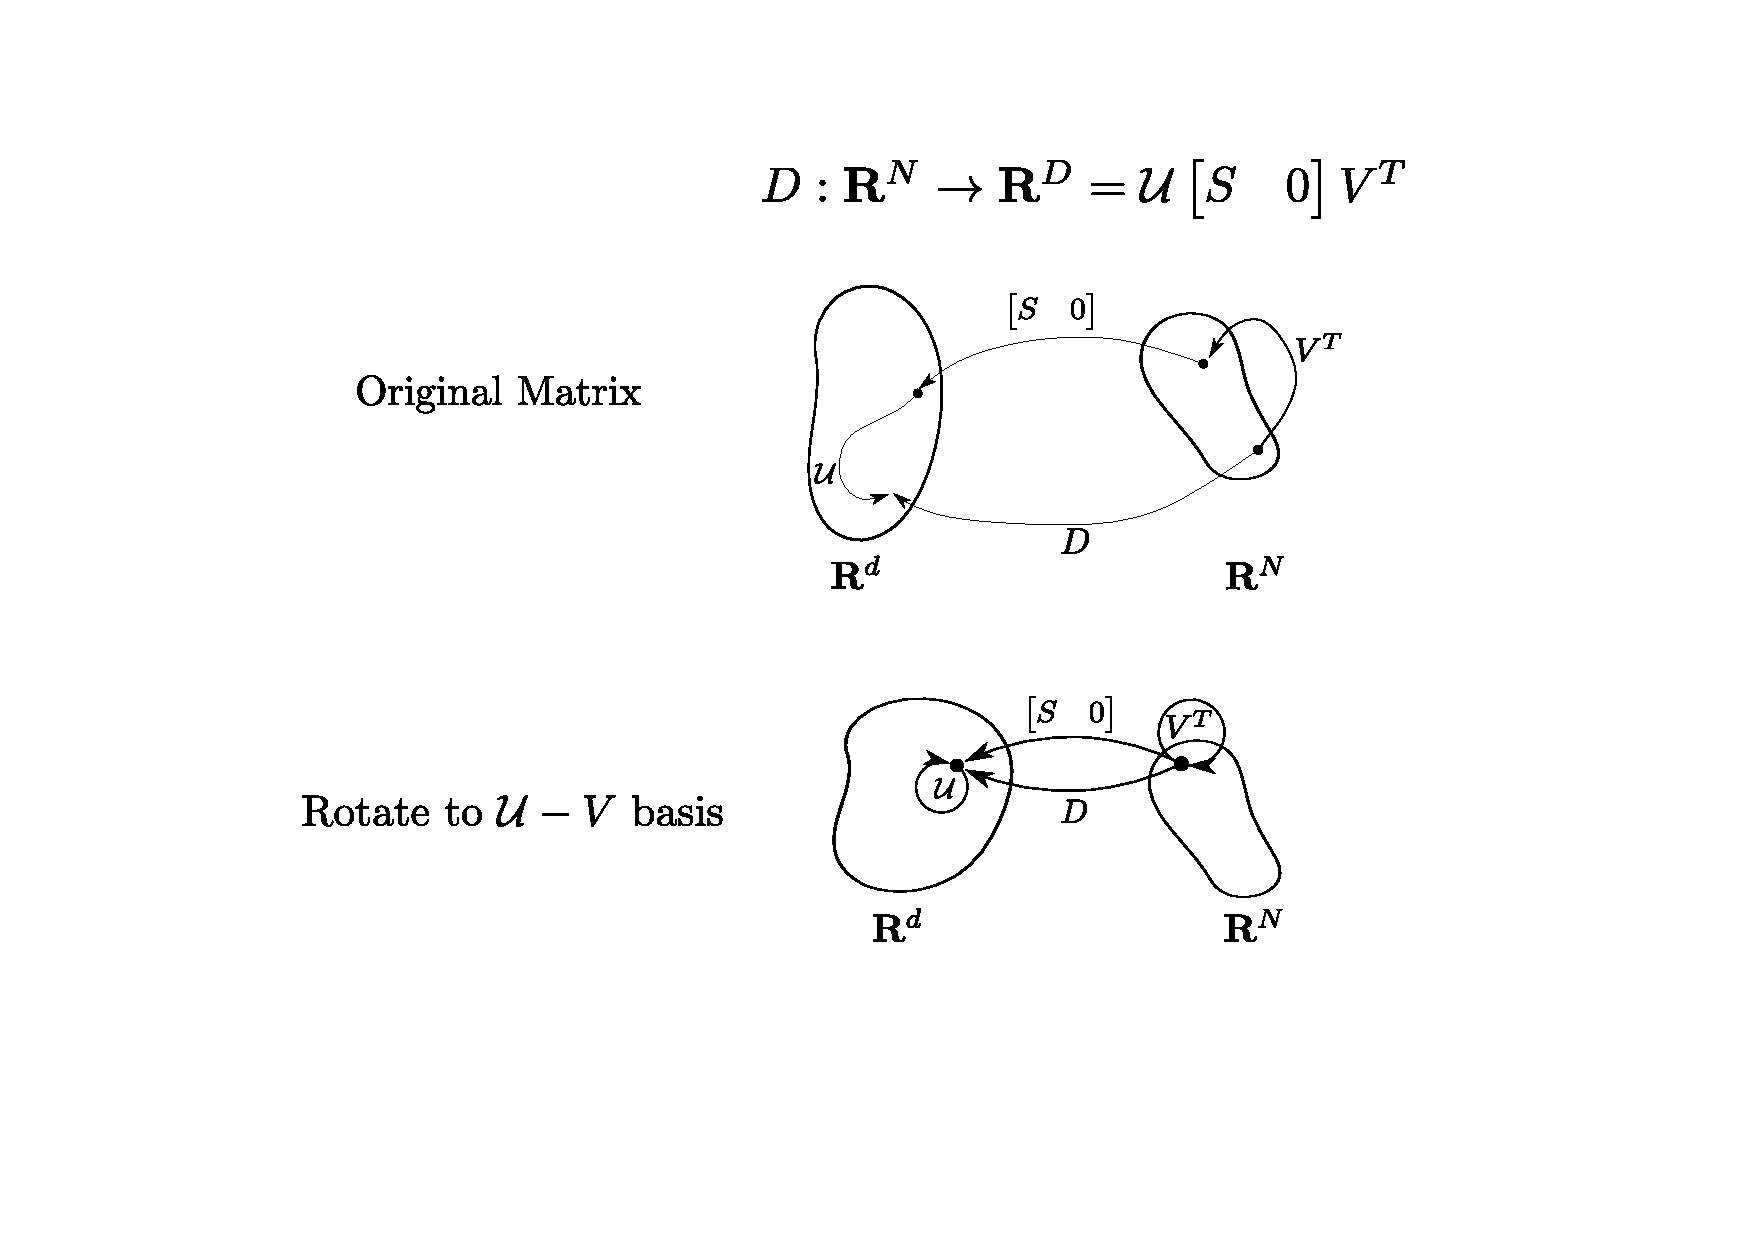
\includegraphics[scale=.6]{figures/linear_map_sequence}
\caption{Visualizing $D$ as a sequence of linear maps between subspaces. \textbf{\textit{Top: }} The matrix $D \in \mathbf{R}^{d \times N}$ is decomposed via SVD into a sequence of 3 linear maps (matrices). The rightmost matrix $V^T \in \mathbf{R}^{N \times N}$ projects a vector  $x$  to give coefficients for the expansion in the basis $V$. The center matrix $\begin{bmatrix} S & 0 \end{bmatrix} \in \mathbf{R}^{d \times N}$ maps vectors from the $V$ basis to a vector in $\mathbf{R}^d$ by scaling and truncation. The leftmost matrix $\mathcal{U} \in \mathbf{R}^{d \times d}$ gives the resultant vector $D x \in \mathbf{R}^d$ by using the scaled vector $\begin{bmatrix} S & 0 \end{bmatrix} V^T$  as coefficients for a basis expansion in $\mathcal{U}$. \textbf{\textit{Bottom:}} We rotate the basis for vectors in $\mathbf{R}^N$ and $\mathbf{R}^d$ to the $\mathcal{U}$ and $V$ bases respectively. This negates the need of $D$ to preemptively project and afterward rotate a vector, leaving only scaling by a diagonal matrix. The mapping $D$ performs on a vector $y$ simplifies to multiplication by a diagonal matrix $S$ of $y$'s first $d$ components. 
}
\label{fig:linear_maps_between_subspaces_D_real}
\end{figure}

\clearpage

\item For the network decoder to fully span the state space of interest, it must have anti-parallel encoding directions even in the rotated orthonormal basis. To do so we augment the rotated bases by adding an antiparallel set so they are no longer orthonormal. We consider two methods of adding antiparallel bases: 

\textbf{\textit{Method A: Separate Antiparallel Networks}} One solution is to form a separate network of $d$ neurons whose encoding directions are the antiparallel set $-\mathcal{U}$. That is, we form an identical network except the decode matrix is
$$ -D = -\mathcal{U} \begin{bmatrix} S & 0 \end{bmatrix} V^T.$$

We then add the output of the two networks to recover the encoded state. 


We divide the error into its positive and negative components and encode each in a separate network. Let
$$
\epsilon^{+} = \epsilon \geq 0,
$$

be the nonnegative component of $\epsilon$. Note that the original estimate, $e$ may contain negative or positive components, but the projection $\epsilon^{+}$ does not.  Similarly define the negative error by 

$$
\epsilon^{-} = -\epsilon < 0.
$$

Note
$$
\epsilon^{-} \neq -\epsilon^+. 
$$
Rather, 
$$
\epsilon = \epsilon^{+} - \epsilon^{-}.
$$

The relationship between $\epsilon^+$ and $\epsilon^-$ resembles two orthogonal subspaces. The preceding relation is analogous to a direct sum. 


Let
$$
v^{+} = S^T \epsilon^+, 
$$
be the voltage induced by projecting $\epsilon^+$ onto the orthonormal bases given by $D = \mathcal{U} \begin{bmatrix} S & 0 \end{bmatrix} V^T$,

and 
$$
v^{-} = S^T \epsilon^-
$$

be the respective projection onto the antiparallel orthonormal bases, $D = \mathcal{U} \begin{bmatrix} -S & 0 \end{bmatrix} V^T$.

Note that
$$
v^{-} \neq -v^+. 
$$
Rather, 
$$
v= v^{+} - v^{-}, 
$$

where $v$ is the voltage of an idealized neuron capable of positive and negative area spikes. Note that both $v_j^+$ and $v_j^-$ are bounded by thresholds $v_{th} = \frac{||S_j||^2}{2}$, so that the idealized neuron is always within the voltage range $v \in \left[ -v_{th}, v_{th} \right]$. This is equivalent to asserting the error along each encoding direction $S_j$ is contained within the polytope $S_j^T \epsilon \leq \frac{||S_j||^2}{2}$. 

Let $\rho^+$ and $\tilde{o}^+$ be the slow synaptic feedback and spike trains of the positive neurons, with $\rho^-$ and $\tilde{o}^-$ defined similarly for the negative neurons. Finally split $\tilde{c} = \tilde{c}^+ - \tilde{c}^-$ into positive and negative components as with $\epsilon$.  

 We now have two $d-$dimensional systems of equations.  
\begin{align*}
\dot{v}^{+}
&= 
\begin{bmatrix}
\Lambda & 0
\\
0 & 0
\end{bmatrix}
v^+ +
\begin{bmatrix}
S \left(\Lambda + I_d \right) S & 0
\\
0 & 0
\end{bmatrix}
  \rho^+
  +
\begin{bmatrix}
S \\ 0
\end{bmatrix}  
\beta \tilde{c}^+
  - 
 \begin{bmatrix}
S^2 & 0
\\
0 & 0
\end{bmatrix}
    \tilde{o}^+,
    \\
    \\
    \dot{v}^{-}
&= 
\begin{bmatrix}
\Lambda & 0
\\
0 & 0
\end{bmatrix}
v^- +
\begin{bmatrix}
S \left(\Lambda + I_d \right) S & 0
\\
0 & 0
\end{bmatrix}
  \rho^-
  +
\begin{bmatrix}
S \\ 0
\end{bmatrix}  
\beta \tilde{c}^-
  - 
 \begin{bmatrix}
S^2 & 0
\\
0 & 0
\end{bmatrix}
    \tilde{o}^-.
\end{align*}


These equations each produce estimates 
$$
\hat{y}^+ = S \rho^+,
$$

$$
\hat{y}^- = S \rho^-,
$$

which give the network estimate

$$
\hat{y} = \hat{y}^+ - \hat{y}^-.
$$



Writing the above as a single network, assume $N = 2d$ so we need not fill with zeros:

$$
\begin{bmatrix}\dot{v}^+\\ \dot{v}^-\end{bmatrix} = \begin{bmatrix}
\Lambda & 0
\\
0 & \Lambda 
\end{bmatrix}
\begin{bmatrix} v^+ \\ v^- \end{bmatrix}
 +
\begin{bmatrix}
S \left(\Lambda + I_{d} \right) S & 0 
\\
0 & S \left(\Lambda + I_{d} \right) S 
\end{bmatrix}
\begin{bmatrix}
  \rho^+
  \\
  \rho^-
\end{bmatrix}
  +
\begin{bmatrix}
S & 0 \\ 0 & S
\end{bmatrix}  
\beta 
\begin{bmatrix}
\tilde{c}^+
\\
\tilde{c}^-
\end{bmatrix}
  - 
 \begin{bmatrix}
S^2 & 0
\\
0 & S^2
\end{bmatrix}
\begin{bmatrix}
    \tilde{o}^+
    \\
    \tilde{o}^-
\end{bmatrix}
.
$$

We simplify this by writing 

$$
   \dot{v}
= 
\Lambda 
v +
S \left(\Lambda + I_{2d} \right) S 
  \rho
  +
S 
\beta \tilde{c}
  - 
S^2 
    \tilde{o}, 
$$


where we have made the following substitutions: 

\begin{align*}
	v &\leftarrow \begin{bmatrix}
	v^+ \\ v^-
	\end{bmatrix} 
	    \in \mathbf{R}^{2 d},
	\\
	\\
	\Lambda &\leftarrow
    \begin{bmatrix}
    \Lambda & 0 \\ 0 & \Lambda
    \end{bmatrix}
    \in \mathbf{R}^{2 d \times 2 d},
    \\
    \\
    S &\leftarrow
    \begin{bmatrix}
    S & 0 \\ 0 & S
    \end{bmatrix}
   \in \mathbf{R}^{2 d \times 2 d},\\
    \\
    \rho &\leftarrow 
    \begin{bmatrix}
    \rho^+ \\ \rho^-
    \end{bmatrix} \in \mathbf{R}^{2d},
    \\
    \\
    \tilde{o} &\leftarrow 
    \begin{bmatrix}
    \tilde{o}^+ \\ \tilde{o}^-
    \end{bmatrix} \in \mathbf{R}^{2d},
    \\
    \\
    \beta &\leftarrow 
    \begin{bmatrix}
    \beta & 0 \\ 0 & \beta
    \end{bmatrix}
    \in \mathbf{R}^{2d \times 2d},
    \\
    \\
    \tilde{c} & \leftarrow 
    \begin{bmatrix}
    \tilde{c}^+ \\ \tilde{c}^-
    \end{bmatrix} \in \mathbf{R}^{2d},
    \\
    \\
    v_{th} &\leftarrow 
    \begin{bmatrix}
    v_{th} \\ v_{th}
    \end{bmatrix} \in \mathbf{R}^{2d}.
\end{align*}

To decode from the network to the $d-$dimensional estimate, we multiply by $ \begin{bmatrix}
\mathcal{U} & -\mathcal{U}
\end{bmatrix} \in \mathbf{R}^{d \times 2d},$ i.e 
$$
\hat{y} = \hat{y}^+ - \hat{y}^- = \begin{bmatrix}
\mathcal{U} & -\mathcal{U}
\end{bmatrix} \rho.
$$
\clearpage



This approach suggests a balance between excitatory and inhibitory neurons when coding an oscillatory signal that inhabits the full $d-$dimensional state space. To illustrate, consider a 2 neuron network as in figure (\ref{fig:ei_balance_demo}). An input $\tilde{c}(\xi) = sin(\omega \xi)$ drives the neurons which encode $v^+$ and $v^-$ respectively. A readout neuron performs leaky integration of the spike trains from the two driven neurons. Consider how a received spike changes the voltage of the readout neuron. A spike from one neuron will increase the readout neuron's membrane potential (excitatory input), while a spike from the other neuron must symmetrically decrease the readout neuron's potential (inhibitory input). In this case, we observe equal levels of excitatory (and inhibitory input from the two neurons, suggesting a tight balance. Note also this ensures consistency with Dale's law, which states that a neuron cannot both excite and inhibit other neurons. 

\begin{figure}
\centering

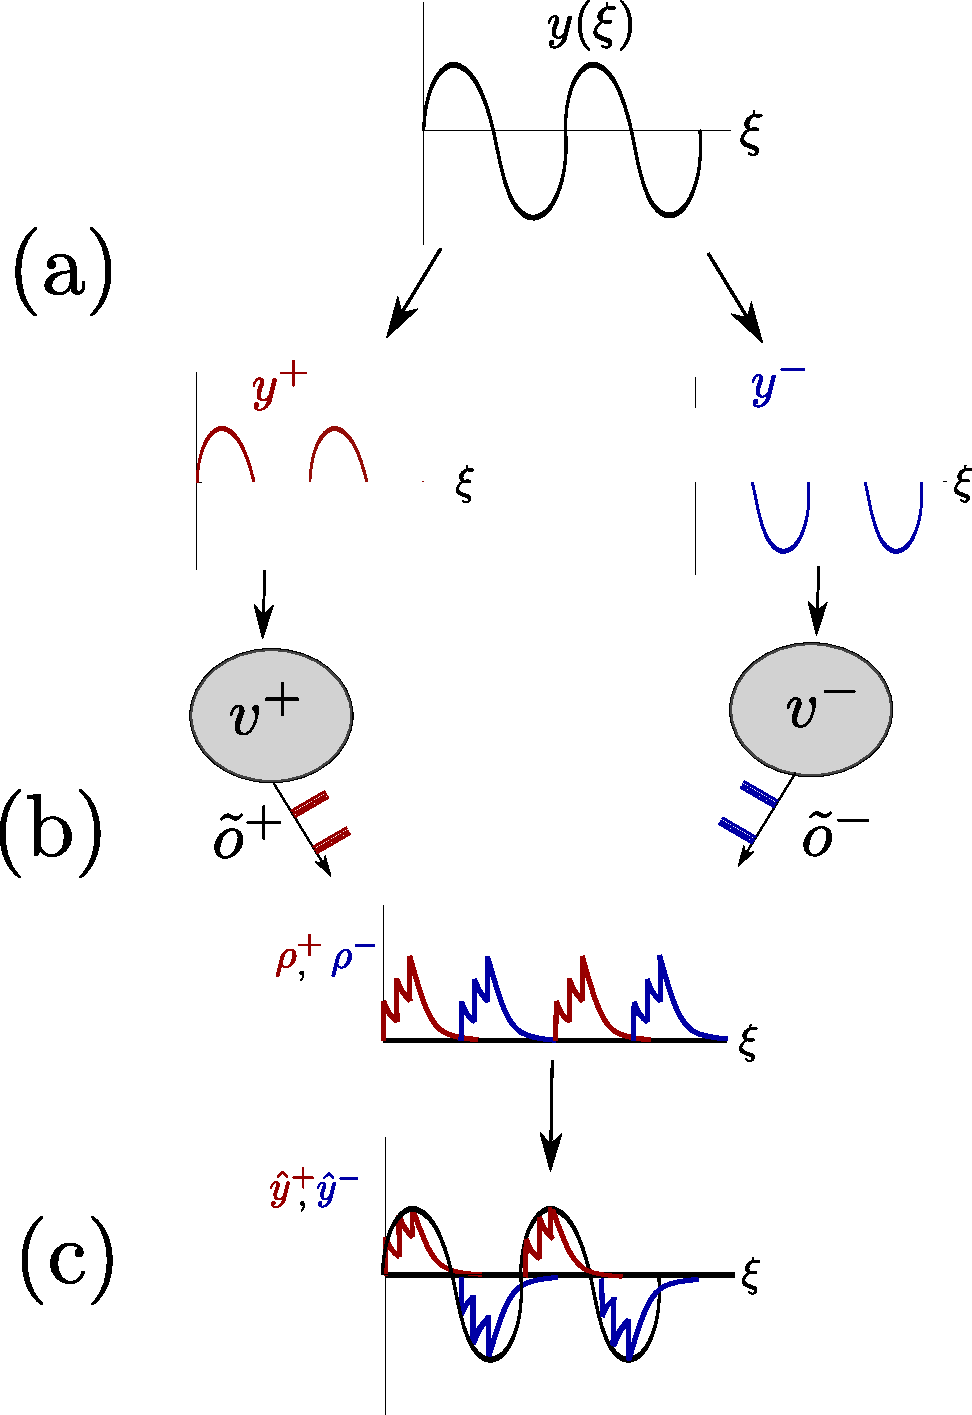
\includegraphics[width=\linewidth, height=19cm]{figures/demo_balance_ei}
\caption{Balance Between Excitatory and Inhibitory Activity for Oscilllatory Input. \textbf{\textit{(a):}} A sinusoidal input $y$ is divided into its positive (excitatory) and negative (inhibitory) components.\textbf{\textit{(b):}} Each neuron encodes its respective input by spiking to produce a nonnegative filtered spike train $\rho$. \textbf{\textit{(c):}} } The network estimate is the sum of activity from excitatory and inhibitory filtered spike trains. For oscillatory input, both neurons must spike in equal amounts so that the amplitude of oscillation remains bounded. 
\label{fig:ei_balance_demo}
\end{figure}


Note also that the fast coupling matrix preceding $\tilde{o}$ is diagonal. This implies that when a neuron $j$ spikes, its antiparallel neuron is unchanged. In the PCF, a neuron spike resets its threshold to $-v_{th}$, but likewise sets a neuron antiparallel to it to $v_{th}$. Next, the antiparallel neuron spikes and likewise resets the neuron. This cycle repeats itself causing the network estimate to oscillate uncontrollably in a catastrophic network failure termed "ping-ponging". The PCF addresses this through regularization terms applied to the network objective $\mathcal{L}$ and added noise,  (Boerlin 2013) both of which are unnecessary in this case. 
\end{enumerate}

\clearpage

\textbf{\textit{Method B: Fast-Coupling Between Antiparallel Neurons}} The other method we consider maintains the fast-coupling relationship between a neuron and its opposite as described in PCF. Fast-coupling implies that when a neuron $i$ with encoding direction $d_i$ spikes, neuron $j$'s voltage changes by $-d_j^T d_i$. This is visible in the spiking ($D^TDo$) term in PCF's voltage equation (\ref{eq:derivation_init}). If $d_j = -d_i$, then a spike in $d_j$ decreases $j$'s voltage by $||d_j||^2$, while simultaneously increasing neuron $i$'s voltage by the same. 

\begin{enumerate}



\item  Previously we used a subset of $d$ neurons from the decoder matrix, 
$$
D = \mathcal{U} \begin{bmatrix}
S & 0
\end{bmatrix}
V^T \in \mathbf{R}^{d \times N}.
$$

In adding $d$ antiparallel neurons, we assume $N \geq 2d$ and instead use $2d$ neurons, i.e. we write
$$
D = \begin{bmatrix}
\mathcal{U} & -\mathcal{U}
\end{bmatrix}^T \begin{bmatrix}
S & 0 & 0
\\
0 & S & 0
\end{bmatrix}
V^T \in \mathbf{R}^{d \times N}.
$$

The first and second $d$ neurons have encoding directions $\mathcal{U}$ and $-\mathcal{U}$ respectively. Before the first $d$ right eigenvectors $V_j$ were scaled by $\sigma_j$ and mapped to $\mathcal{U}_j$, with the remaining $V_j$ mapped to $0$. In adding $d$ antiparallel vectors, we scale an additional $d$ right eigenvectors $V_{j+d}$ by $\sigma_j$ and map them to $-\mathcal{U}_j$. 


The dynamical system remains the same, i.e.
\begin{align*}
\dot{y} &= \Lambda y + \beta \tilde{c}. 
\end{align*}






\item The network estimation 
$$
\hat{y}  = \mathcal{U}^T D \hat{x} = \begin{bmatrix}
S & 0
\end{bmatrix} \rho
$$
is now

\begin{align*}
\hat{y} &= \mathcal{U}^T \begin{bmatrix}
\mathcal{U} & -\mathcal{U}
\end{bmatrix}
\begin{bmatrix}
S & 0 & 0 
\\
0 & S & 0
\end{bmatrix}
\rho
\\
\\
&=
\begin{bmatrix}
S & -S & 0
\end{bmatrix}
\rho.
\end{align*}


We rederive the error dynamics 
\begin{align*}
\dot{\epsilon} &= \dot{y} - \dot{\hat{y}}
\\
\\
&=
\Lambda 
y
+ \beta
\tilde{c}
-
\begin{bmatrix}
S & -S & 0
\end{bmatrix}
\left( -\rho + \tilde{o}\right)
\\
\\
&= 
\Lambda 
\left(\epsilon + \hat{y} \right)
+
\begin{bmatrix}
S & -S & 0
\end{bmatrix}
\rho
+ \beta
\tilde{c}
-
\begin{bmatrix}
S & -S & 0
\end{bmatrix}
\tilde{o}
\\
\\
&=
\Lambda 
\epsilon 
+
\left(I + \Lambda\right)
\begin{bmatrix}
S & -S & 0
\end{bmatrix}
\rho
+ \beta
\tilde{c}
-
\begin{bmatrix}
S & -S & 0
\end{bmatrix}
\tilde{o}
\end{align*}

\item We previously obtained voltage by optimizing the objective

$$
\mathcal{L} = ||y - \hat{y}||^2. 
$$


For the first $d$ neurons this was 

$$
v_j = S_j^T \epsilon \hspace{3mm}  \text{ if } j \in \left[1, \hdots, d\right].
$$

We now add an addition $d$ neurons with antiparallel directions. For each neuron $j$ we add an additional neuron $j + d$ with oppositve encoding direction, and therefore opposite voltage. The voltage is now 

$$
\begin{cases}
v_j = 
S_j^T \epsilon & \text{ for } j \in \left[1, \hdots, d \right]
\\
-S_{j-d}^T \epsilon & \text{ for } j \in \left[d+1, \hdots, 2d \right]
\end{cases}.
$$

In matrix form, 

$$
v = 
\begin{bmatrix}
S
\\
-S
\end{bmatrix}\epsilon.
$$


From the error dynamics above, we get

\begin{align}
\label{eq:expanded_voltage_dynamics}
\dot{v} &= 
\begin{bmatrix}
\Lambda  & 0
\\
0 & \Lambda 
\end{bmatrix} 
v
+
\begin{bmatrix}
S
\\
-S
\end{bmatrix} \left(I + \Lambda\right)
\begin{bmatrix}
S & -S & 0
\end{bmatrix}
\rho
+ \begin{bmatrix}
S
\\
-S
\end{bmatrix} \beta
\tilde{c}
-
\begin{bmatrix}
S^2 & -S^2 & 0
\\
-S^2 & S^2 & 0
\end{bmatrix}
\tilde{o}.
\end{align}

Equation (\ref{eq:expanded_voltage_dynamics}) gives the voltage dynamics of $2d$ neurons. 

\item To facilitate comparison between the self-coupled network and original PCF model, we will use this method (B) hereafter. Method A is a viable alternative, however it is fundamentally different than the original PCF model because antiparallel neurons do not interact in contrast with PCF and method B.  We investigate method A later. 
\end{enumerate}


\clearpage

\subsection{Simulation of Basic Equations}
Here we simulate the above equations (\ref{eq:rotated_voltage_dynamics}) and (\ref{eq:rho_dot}) with the $N = 2d$ neurons. The parameters are
\begin{align}
\label{eq:sim_I_params}
A
&=
\ -\begin{bmatrix}  
1 & 0 \\
0 & 1
\end{bmatrix} = \mathcal{U} \Lambda \mathcal{U}^T \notag,
\\
\notag
\\
B
&=
\begin{bmatrix}  
1 & 0 \\
0 & 1
\end{bmatrix}, \notag 
\\
\notag 
\\
c(\xi) 
&=
\begin{bmatrix} 
cos(\frac{\pi}{4} \xi)\\
sin(\frac{\pi}{4} \xi)
\end{bmatrix} 
\\
\notag
\\
D
&=
\mathcal{U} 
\begin{bmatrix}
S & 0
\end{bmatrix}
V^T
=
\mathcal{U} 
\begin{bmatrix}
.1 \, I_d & 0
\end{bmatrix}
I_N \notag,
\\
\notag 
\\
d\xi 
&= 
10^{-6}, \notag 
\\
\notag 
\\
N 
&= 
4,\notag 
\\
\notag 
\\
x(0) 
&= 
\begin{bmatrix} \frac{1}{2} & \frac{1}{2} \end{bmatrix}.\notag 
\end{align}

\begin{figure}
    \centering
    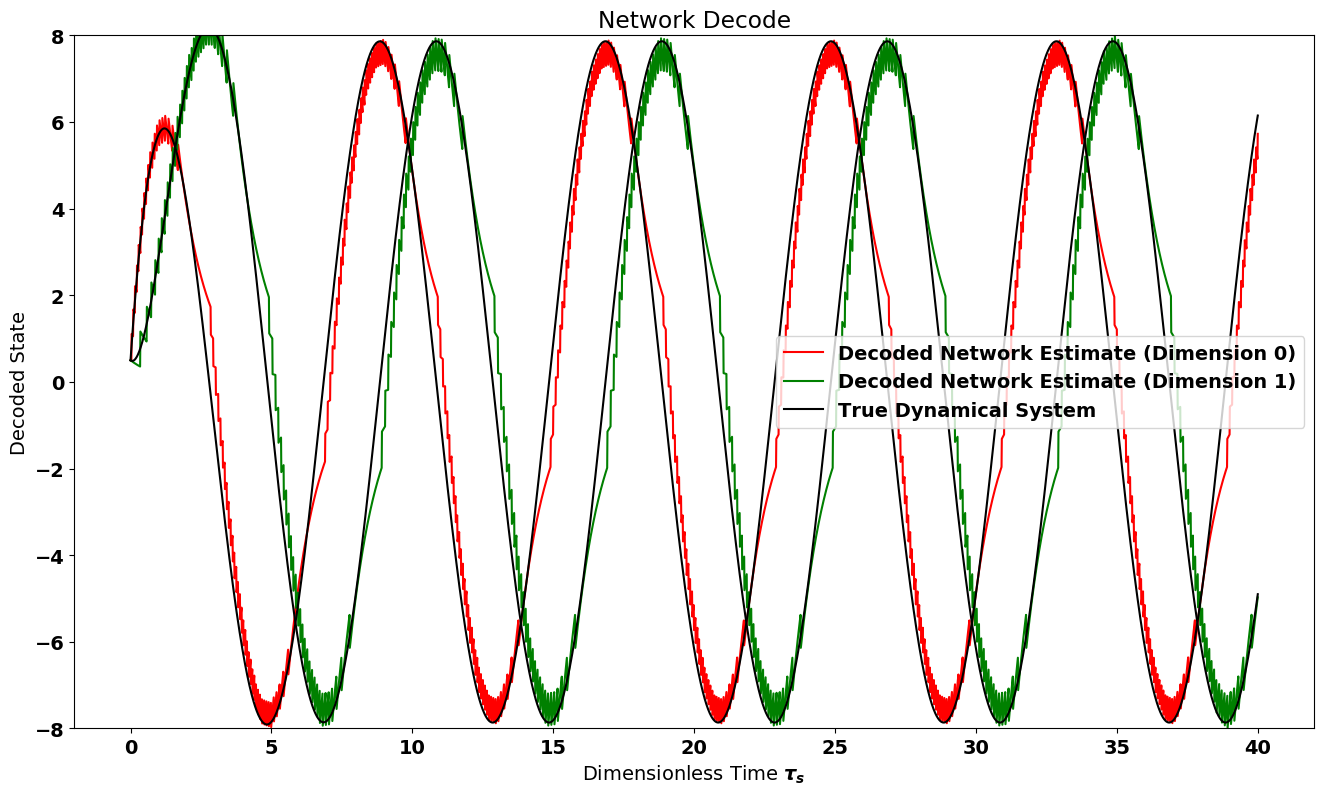
\includegraphics[width=.75\linewidth]{figures/network_decode.png}

    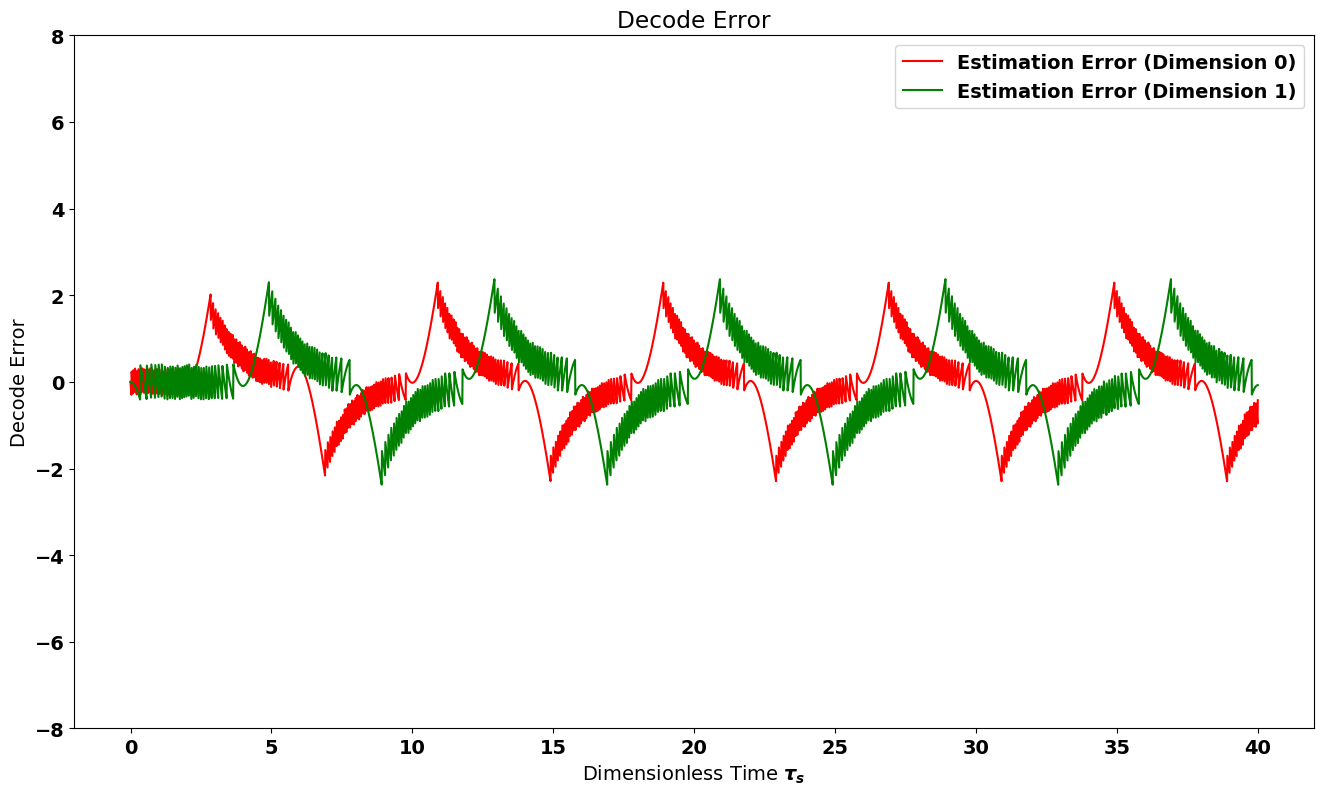
\includegraphics[width=.75\linewidth]{figures/decode_error.png}

    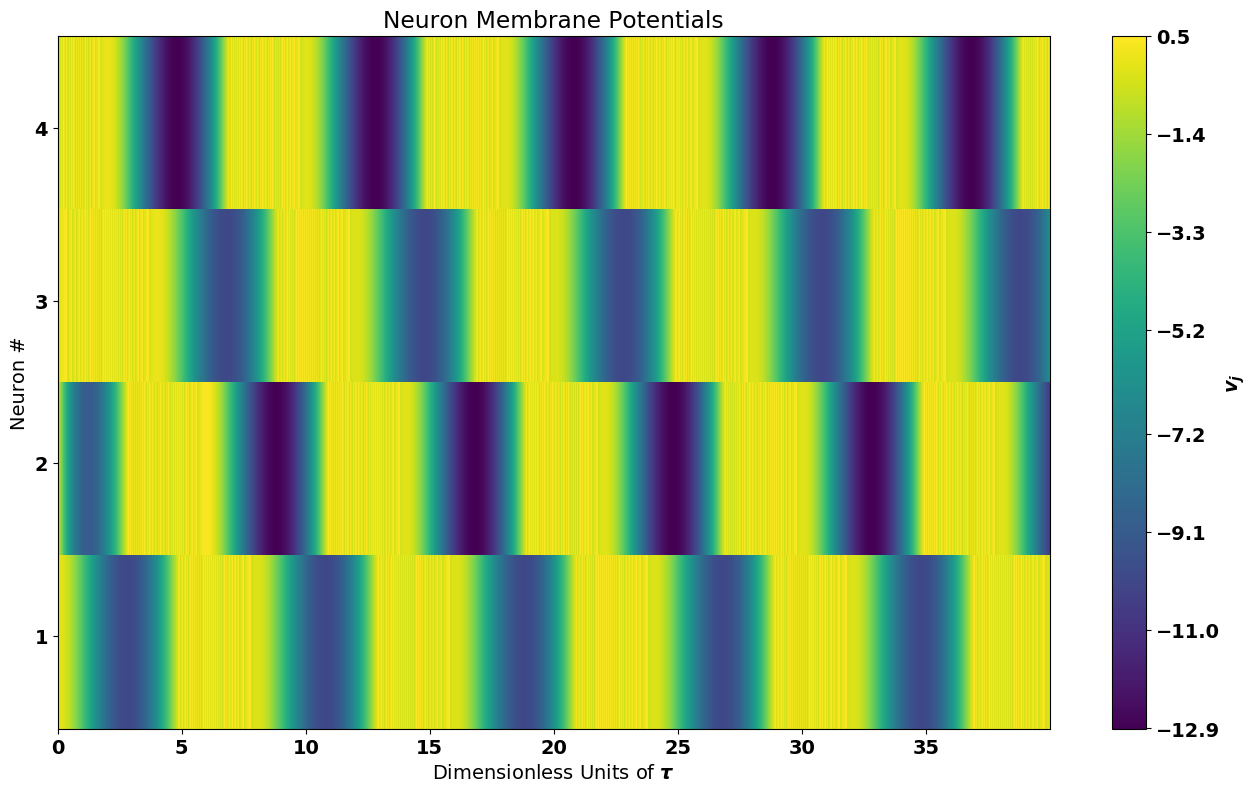
\includegraphics[width=.7\linewidth]{figures/membrane_potential_image.png}
\end{figure}

\newpage

\captionof{figure}{Simulation of equations (\ref{eq:rotated_voltage_dynamics}) and
    (\ref{eq:rho_dot}) with parameters listed in equation (\ref{eq:sim_I_params}). \textbf{\textit{Top:}} The decoded network estimate plotted alongside the target dynamical system. \textbf{\textit{Middle:}} The estimation error along each state-space dimension. \textbf{\textit{Bottom: }}The membrane potentials of the 4 neurons during the same time period.\\
    For the numerical implementation, the matrix exponential was used to integrate the continuous terms over a simulation time step. Continuous terms include all equation terms excepting the delta functions $\omega$ handled separately. After integrating over a timestep, any neuron above threshold was manually reset (action of fast inhibition). If multiple neurons are above threshold, the system is integrated backwards in time until only one neuron is above threshold before spiking. The matrix exponential was computed using a Pad\'{e} approximation via the Python package Scipy: \textit{scipy.linalg.expm()}. 
    } 
    \label{fig:Simulation_I}